%%%%%%%%%%%%%%%%%%%%%%%%%%%%%%%% 
\section{The Fine-Grained Tracker} 
\label{cdrsec:detectors-nd-ref-fgt}

The scope of the DUNE Fine-Grained Tracker (FGT) near neutrino detector includes the design, procurement, fabrication, testing, delivery and installation of all the systems and components that comprise it:

%\fixme{edit this as needed}

\begin{itemize}
\item a central straw-tube tracker (STT)
\item an electromagnetic calorimeter (ECAL) 
\item a 0.4-T dipole magnet surrounding the STT and ECAL
\item muon identifiers (MuIDs) located in the steel of the magnet, as well as upstream and downstream of the STT
\item instrumentation for monitoring and control
\end{itemize}



\begin{cdrfigure}[A schematic drawing of the fine-grained
tracker design]{STT_schematic}{A schematic drawing of the fine-grained tracker design.}
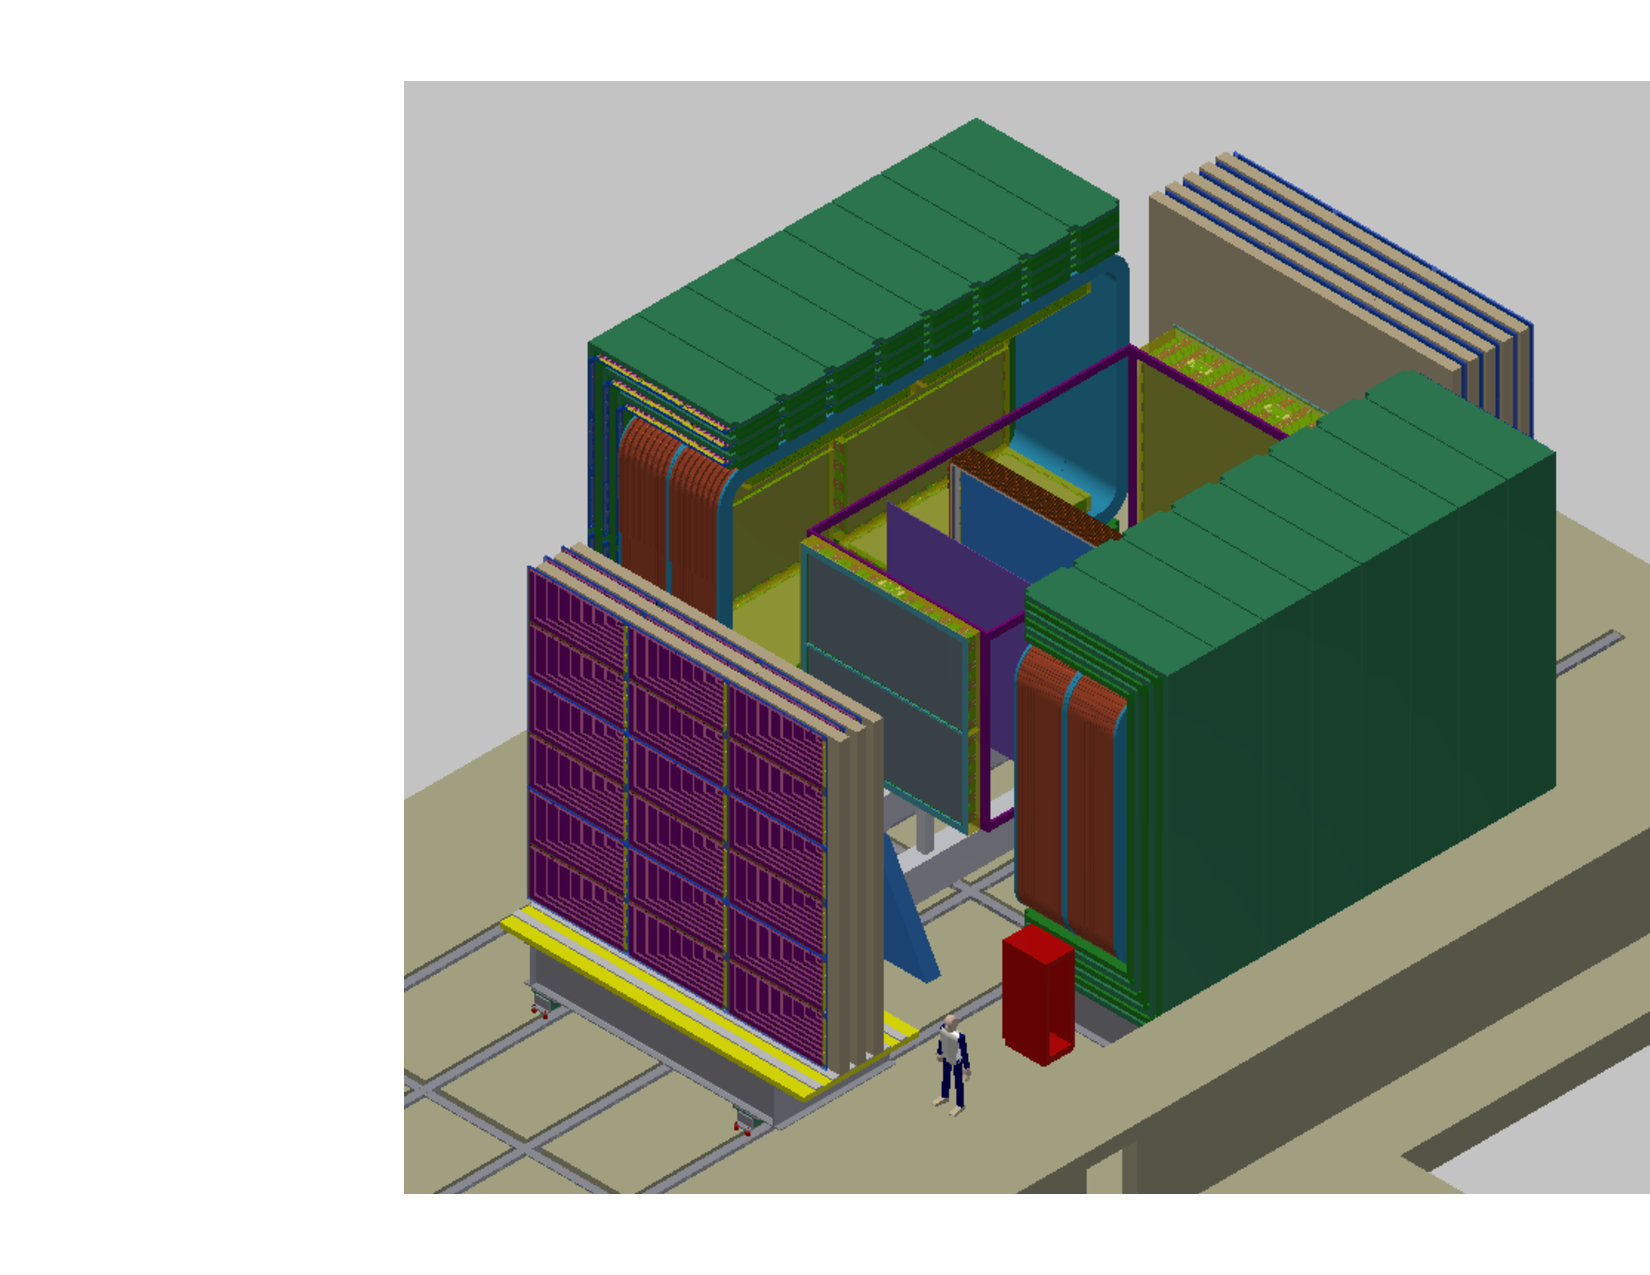
\includegraphics[width=\textwidth]{FGT_Overview}
\end{cdrfigure}

A schematic drawing of the FGT design is shown in Figure~\ref{fig:STT_schematic}. 
The design presented here meets the required performance for making precision measurements of the 
neutrino fluxes, cross sections, signal rates and background rates for the DUNE far detector. 
The DUNE ND must fulfill the physics program described in Section~\ref{ch:physics-nd}, as well 
as in Ref.~\cite{DPR}. The most significant requirements~\cite{ND-REQ1,ND-REQ2} for the FGT include:  

\begin{itemize}
\item low density $\rho \sim 0.1$ g/cm$^3$, similar to that of liquid hydrogen

\item dipole magnetic field of $B=0.4$ T with high detector granularity 

\item excellent momentum and angular resolutions for $\mu^{\pm}$, $e^{\pm}$, 
$\pi^{\pm}$ and $proton$, and $\pi^0$/$\gamma$ via decay/conversion, 
 and $K^0_S$/$\Lambda$ produced in $\nu$-induced interactions

\item 4$\pi$ ECAL coverage to ensure an  
 accurate determination of the momentum vector of the hadronic shower

\item 4$\pi$ MuID coverage to identify muons with a wide range of energies and angles  

\item excellent electron/positron identification through the use of transition radiation (TR) 

\item $\pi/K/p$ identification by dE/dx 

\item use of a variety of nuclear targets, (C$_3$H$_6$)$_n$, Ar, Ca, C, Fe, etc., to quantitate the impact of nuclear 
effects in $\nu$($\bar \nu$)-nucleus cross sections  

\item provide more than 10 times the unoscillated statistics expected in a 40 kt FD on Ar target

%\item  identification and measurement of processes such as neutral current $\pi^0$ production that can mimic oscillation signals at the FD
%\item comparability with measurements made in the FD
%\item measurement of nuclear effects, including short-range correlations, two-body currents, pion absorption, initial-state interactions, 
%and final-state interactions
\end{itemize}
Regardless of the process under study, the goal is
to have the systematic error less than the corresponding statistical error. A summary of the performance
requirements is given in Table~\ref{tab:comparison}

%The FGT will measure the neutrino event rates and cross sections 
%on argon, water, and other nuclear 
%targets for both $\nu_e$ and $\nu_\mu$ charged current (CC) and
%neutral current (NC) scattering events. The FGT design 
%consists of a straw-tube tracker (STT), consisting of straw tubes, water targets, argon targets, 
%and radiator targets, and an electromagnetic calorimeter (ECAL), both inside a
%dipole magnet. In addition, muon detectors (MuID) consisting of resistive plate
%chambers (RPCs) will be embedded in the steel
%of the magnet. 

\begin{cdrtable}[A summary of the performance for 
the FGT configuration]{ll}{comparison}{A summary of the performance for 
the FGT configuration}
Performance Metric&FGT\\ \toprowrule
Straw Tube Detector Volume & 3.5m x 3.5m x 6.4m \\ \colhline
Straw Tube Detector Mass&8~t ($\rho \sim 0.1$ g/cm$^3$)\\ \colhline
Vertex Resolution&0.1 mm \\ \colhline
Angular Resolution&2 mrad \\ \colhline
$E_e$ Resolution&5\% \\ \colhline
$E_\mu$ Resolution&5\% \\ \colhline
$\nu_\mu/\bar \nu_\mu$ ID&Yes \\ \colhline
$\nu_e/\bar \nu_e$ ID&Yes \\ \colhline
NC$\pi^0$/CCe Rejection&0.1\% \\ \colhline
NC$\gamma$/CCe Rejection&0.2\% \\ \colhline
CC$\mu$/CCe Rejection&0.01\% \\
\end{cdrtable}


%%%%%%%%%%%%%%%%% 
\subsection{Straw-Tube Tracking Detector}
\label{cdrsec:detectors-nd-ref-fgt-stt}

\subsubsection{Straw Tubes} 

The Straw-Tube Tracking Detector (STT) at the center of the FGT 
will be composed of straw tubes with an outer diameter of 1~cm, as well as 
radiators and targets that reside next to the straw tubes (see Figure~\ref{fig:STT_Detail}).
The straw walls are made by wounding together a film of carbon loaded Kapton XC (inner) and 
a film of aluminum coated Kapton HN (outer), for a total thickness of about 70 $\mu$m. 
Vertical (YY) and horizontal (XX) planes of straws will be alternated and 
arranged in modules, with each module containing close-packed double straw layers 
of vertical and horizontal straws (XXYY). 
Figure~\ref{fig:STT_Detail} shows a schematic drawing of an STT module with four straw-tube planes and
radiators. 

\begin{cdrfigure}[A schematic drawing of the fine-grained
tracker design]{STT_Detail}{A schematic drawing of the fine-grained tracker design.}
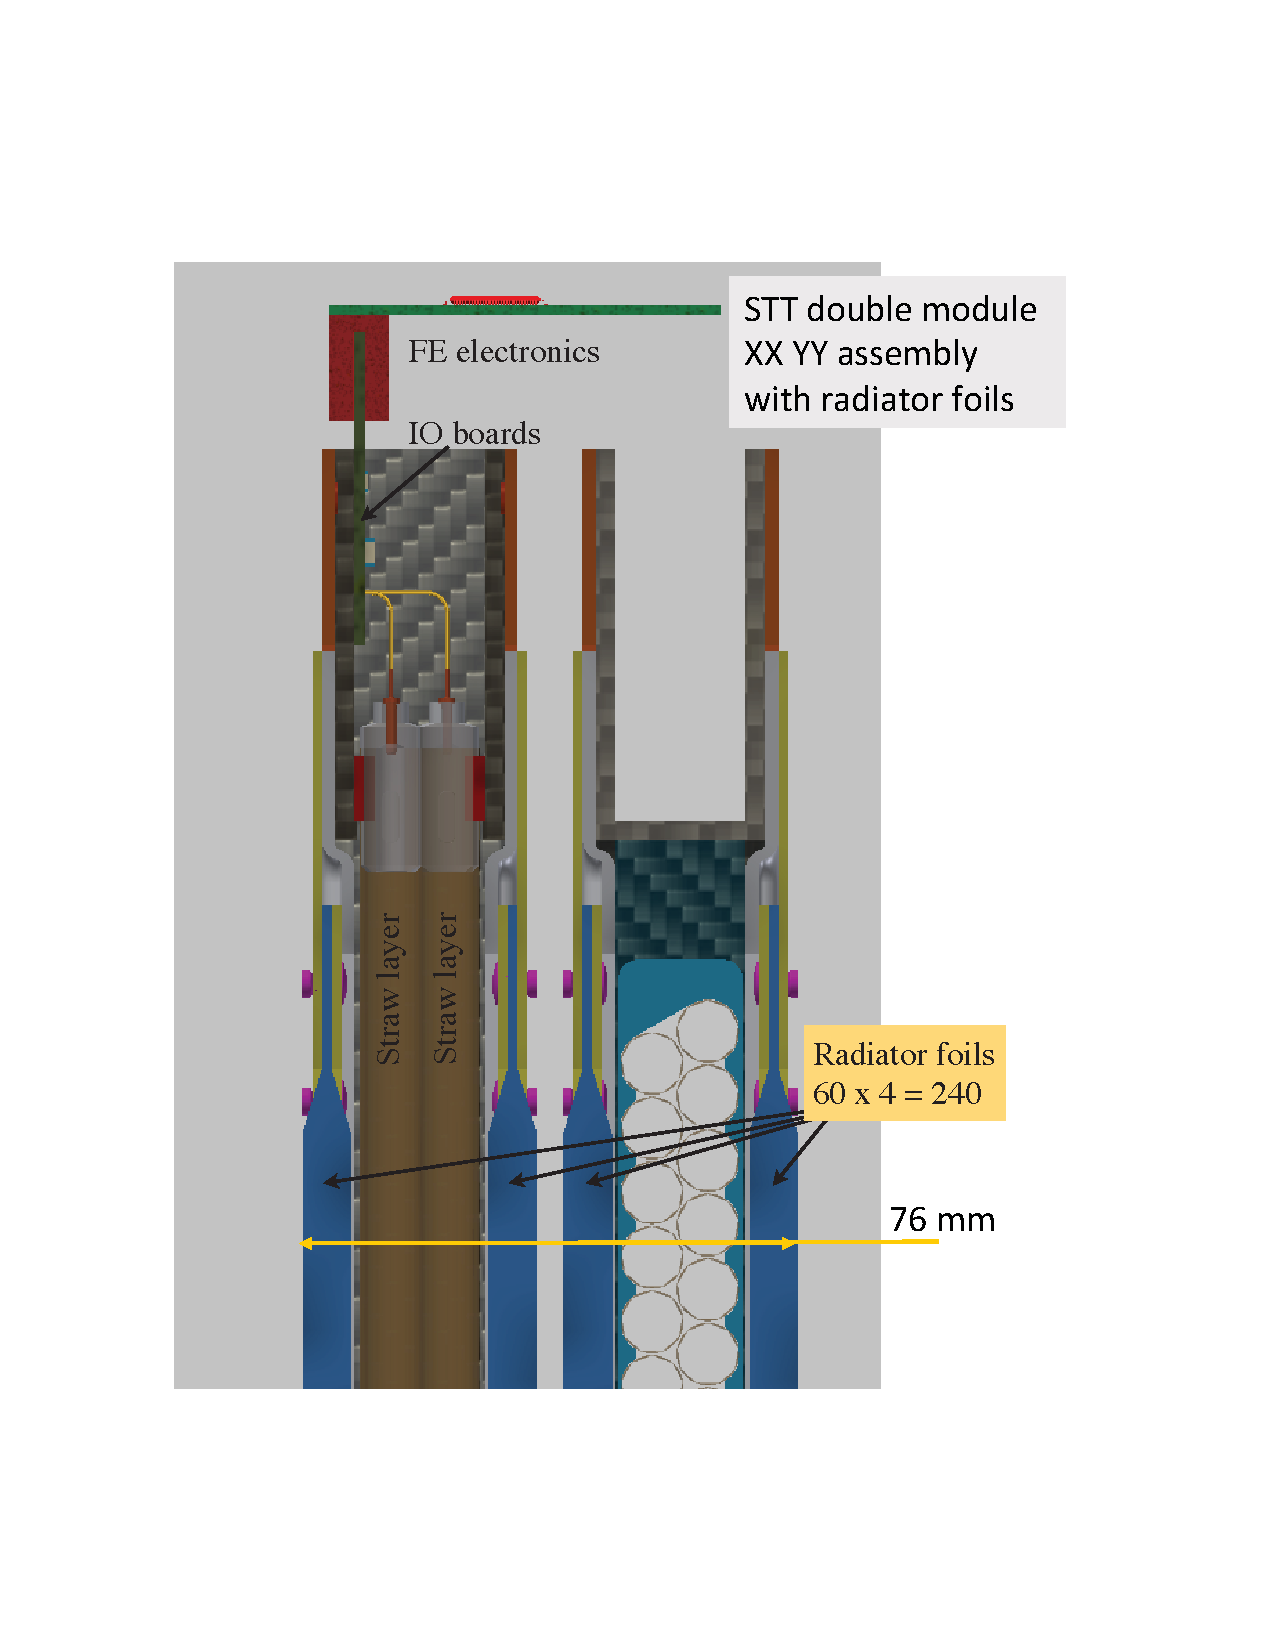
\includegraphics[width=0.5\textwidth]{STT_Detail}
\end{cdrfigure}

The straw tubes will be filled with a
gas mixture of either 70\% Ar plus 30\% CO$_2$ (for modules with targets) or
70\% Xe plus 30\% CO$_2$ (for modules with radiators). 
The dimensions of each module in the reference design will
be approximately 350~cm $\times$ 350~cm $\times$ 8.0~cm, including 
target or radiator planes and four straw planes. For ease of construction and
transportation, each module is made up of four sub-modules, with dimensions of
appproximately 350~cm $\times$ 175~cm $\times$ 4.0~cm. 
%The straw tubes in a single sub-module will be able to provide the tension 
%for the wires, however, a temporary sub-module carbon composite frame will 
%be employed for shipping. 
The sub-modules will be assembled %put together into modules 
at Fermilab, where each module will have a new carbon composite frame around 
the perimeter of the module for support and will have an attached target or 
radiator. 
%Nominally, there will be 34 modules with targets and 46 modules 
%with radiators, still keeping the 
%average density of the STT at around 0.1 g/cm$^3$. 

The modularity of the STT provides for successive measurements using
thin nuclear targets (thickness $< 0.1 X_0$), while the excellent
angular and space resolution allows a clean separation of events
originating in different target materials.

The STT will have a total of 107,520 straws  --- corresponding to 336 straws per plane,
1344 straws per module ---
and 80 modules. Both ends of the straw tubes will be read out, leading to a total
number of electronics channels of 215,040. The total mass of the STT, including targets and radiators, is approximately 8~t.  

\subsubsection{Radiator Targets} 


Radiators will be placed in the downstream STT modules
and will serve as targets for both neutrino interactions 
and Transition Radiation (TR) production. Each STT module contains 
four radiators, where each radiator consists of
60 layers of 25-$\mu$m polypropylene (C$_3$H$_6$)$_n$ 
foils, which are embossed to keep 125-$\mu$m air gaps between 
consecutive foils. 
The mass of each radiator is $\sim17$ kg and the thickness is 
$\sim9$ mm. The use of thin plastic foils regularly spaced allows 
the emission of transition radiation for electron/positron identification, 
which is detected by the Xe gas in the straws. 
% 
The plastic radiators account for about 83\% of the mass of each STT module and 
also provide the main (anti)neutrino target. Overall, a radiator mass of about 5 tons 
is required to achieve the physics sensitivity discussed in Section~\ref{ch:physics-nd} 
and in Ref.~\cite{DPR}. 

\subsubsection{Nuclear Targets} 

The most important nuclear target is the argon target that comprises the DUNE far detector.
This target will consist of planes of 0.5-inch diameter, 3.5-m-long aluminum tubes filled
with argon gas pressurized to 140 atm ($\rho = 0.233$), with sufficient Ar mass to provide 
$\sim$10 times the unoscillated statistics expected in a 40t FD. 

In this regard, a crucial target is calcium which has the same atomic weight ($A=40$) 
as argon but is isoscalar. 
Since most nuclear effects depend on the atomic weight
$A$, inclusive properties of (anti)neutrino interactions are expected
to be the same for these two targets.
This fact would allow the use of both targets to model signal and
backgrounds in the LBNE far detector (argon target), as well as to
compare LBNE results for nuclear effects on argon with the extensive
data on calcium from charged lepton scattering. 


An equally important nuclear target is carbon (graphite), which is essential in order to
get (anti)neutrino interactions on free proton, through a statistical
subtraction procedure from the main polypropylene target (C$_3$H$_6$)$_n$. 
The availability of such a free-proton target will allow 
accurate flux determinations and cross section measurements, and, for the first time, 
a direct model-independent measurement of nuclear effects --- including
both the primary and final-state interactions --- on the argon target
relevant for the far detector oscillation analysis. The required carbon target mass 
is about 0.5~t (in addition to the carbon in the STT frames).  

A stainless steel target in the form of a single thin slab will provide 
service measurements of (anti)neutrino cross-sections for the INO experiment in India. 

Finally, the same aluminum tubes used for the pressurized Ar gas can be filled with 
standard and heavy water (H$_2$O and D$_2$O). The statistical subtraction of H$_2$O from 
D$_2$O would result in a quasi-free neutron. 



%%%%%%%%%%%%%%%%% 
\subsection{Electromagnetic Calorimeter}
\label{cdrsec:detectors-nd-ref-fgt-ecal}

An electromagnetic calorimeter 
(ECAL) will surround the tracking volume on all sides and consist of three separate pieces: Forward ECAL, Barrel ECAL, and Backward ECAL.  
The ECAL conceptual design consists of 
layers of either 1.75-mm-thick (for the forward ECAL) or 3.5-mm-thick 
(for the barrel and backward ECAL) lead sheets and 2.5-cm-wide by 10-mm-thick 
plastic scintillator bars,
as shown in Figure~\ref{fig:ECAL_detail}. 
The scintillator layers for the
Forward and Backward ECAL alternate as XYXYXY..., while the scintillator 
layers for the Barrel ECAL are all horizontal along the axis of the magnet.
The Forward ECAL will consist of 60 layers of scintillator bars, where each
bar has dimensions 3.2~m $\times$ 2.5~cm $\times$ 1~cm. The
Backward ECAL will consist of 16 layers of scintillator bars, where each 
bar has the same dimensions, 3.2~m $\times$ 2.5~cm $\times$ 1~cm. The Barrel ECAL will also consist 
of 16 layers of scintillator bars, where each bar has the same dimensions, 
3.2~m $\times$ 2.5~cm $\times$ 1~cm. 

The lead sheets and scintillator bars will be assembled and glued together
into complete modules of dimension 
3.2~m $\times$ 3.2~cm $\times$ 81~cm for the Forward ECAL and
3.2~m $\times$ 3.2~cm $\times$ 27.5~cm for the Backward ECAL. For the Barrel ECAL, the module 
dimensions will also be 
3.2~m $\times$ 3.2~cm $\times$ 27.5~cm. Two Barrel modules are placed end-to-end 
along the sides of the inner surface of the magnet (eight Barrel modules
total) to provide full coverage of the barrel region.
The total numbers of scintillator bars in the
Forward, Backward, and Barrel ECAL are 7,680, 2,048, and 16,384, respectively, 
for a total of 26,112 bars. 

The scintillator bars will be extruded with 
holes in the middle of each bar. The
holes will then be fitted with 0.7-mm-diameter Kuraray wavelength-shifting (WLS) fibers.
The fibers will be read out by SiPM (silicon photomultiplier) photosensors at each end.
The total mass of scintillator is 20.9~t, 
the total mass of Pb is 70.8~t, and
the total number of readout channels is 52,224. 

\begin{cdrfigure}[Schematic drawing of the ECAL]{ECAL_detail}{Schematic drawing of the ECAL, which is made up of alternating planes
of plastic scintillator and Pb sheets.}
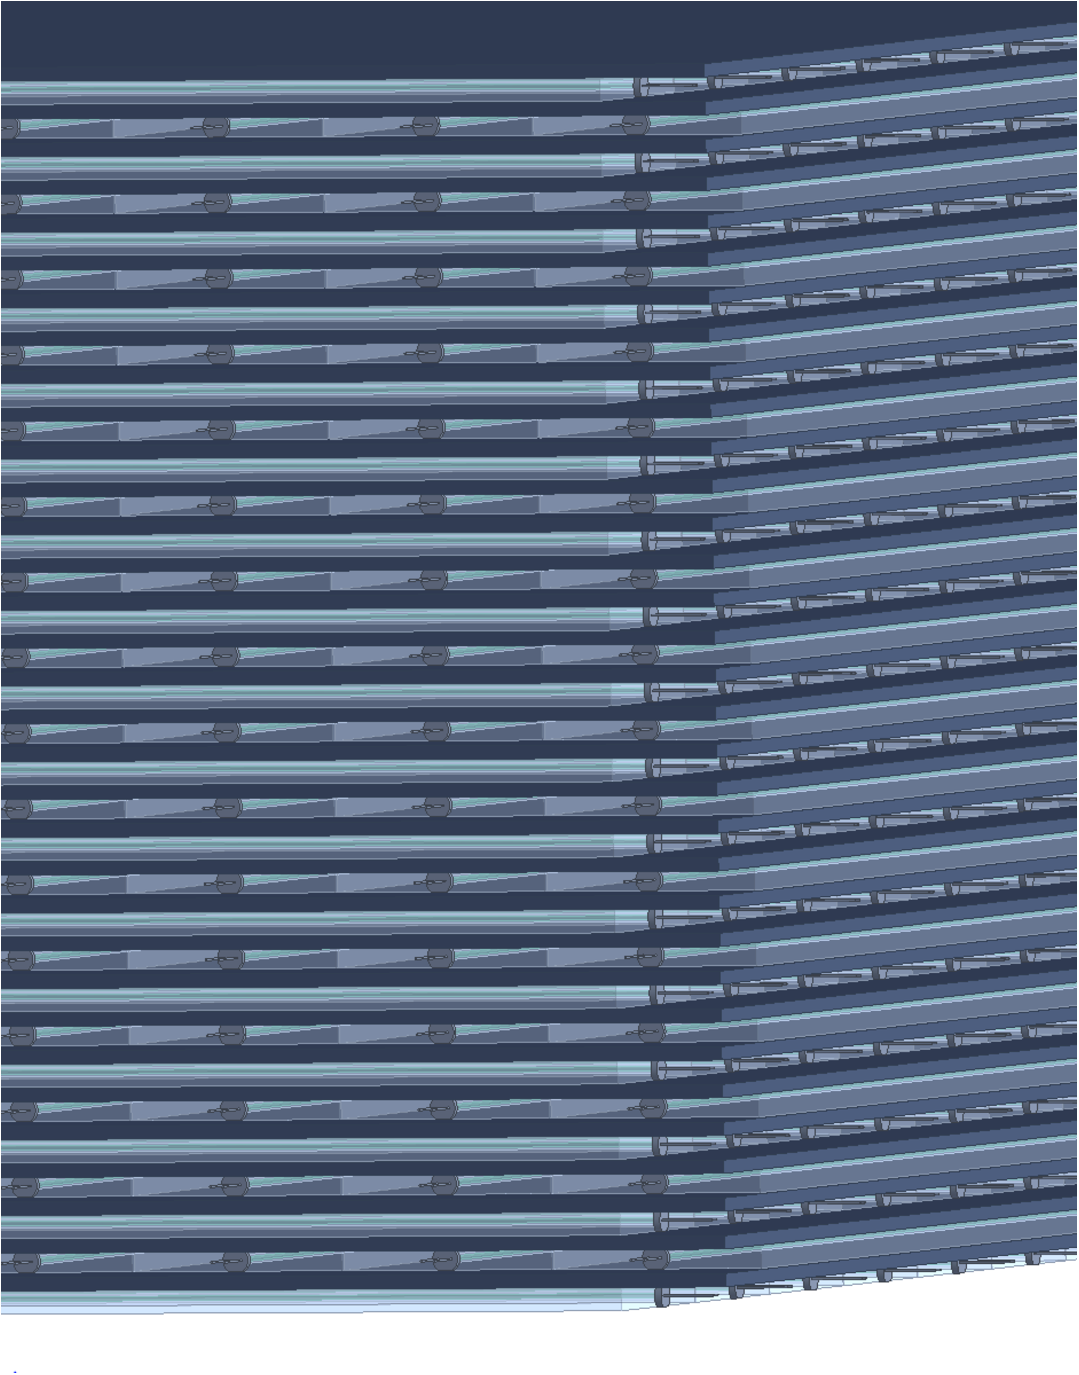
\includegraphics[width=0.5\textwidth,angle=0]{ECAL_detail}
\end{cdrfigure}


%%%%%%%%%%%%%%%%% 
\subsection{Dipole Magnet}
\label{cdrsec:detectors-nd-ref-fgt-magnet}

The STT and ECAL modules will reside inside a 0.4-T dipole 
magnet for the measurement of particle momentum and charge. 
The magnet will have inner dimensions (inside the coils) 
4.5-m wide $\times$ 4.5-m high $\times$ 8.0-m long. The 
magnet has four vertical Al coils, stacked horizontally, producing a horizontal magnetic 
field. The return yoke will be divided into two halves along the 
longitudinal center line to allow the magnet to be opened to service the
detector inside. %, as shown in Figure~\ref{fig:STT_schematic}. 
Each half yoke will be built
from eight ``C'' (C-shaped) sections, and the thickness of the 
magnet steel will be 60~cm, consisting of 6
$\times$ 10-cm-thick plates. The magnet power requirement with Al coils is $\sim 2.4$~MW,
corresponding to 6~kA at 400~V. The water flow required for cooling is 20~l/s.

\begin{cdrfigure}[Magnetic field maps]{Magnet_Bfield}{Design of the dipole magnet and simulation of the 
corresponding magnetic field at the Bhabha Atomic Research Center (BARC) in India.}  
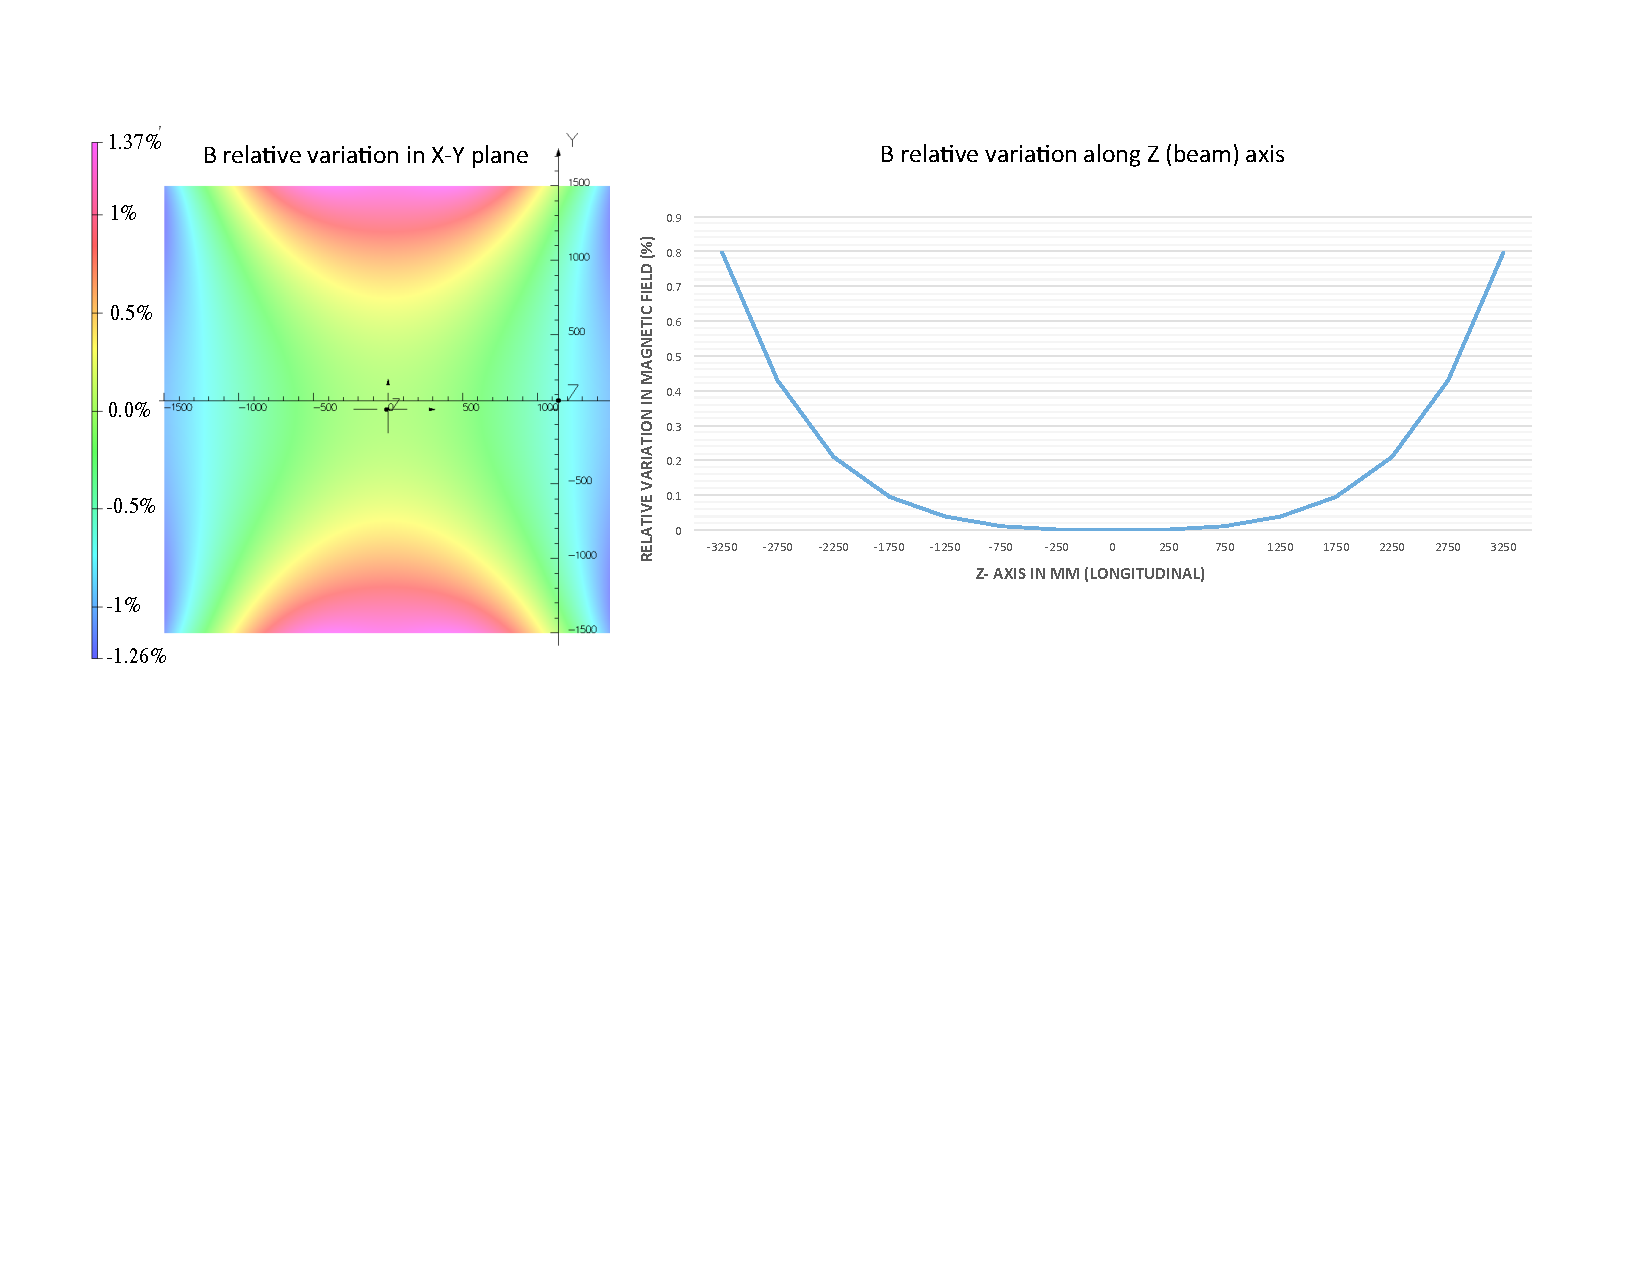
\includegraphics[width=\textwidth]{Magnet_Bfield} % [width=6in,angle=90] <-- was too small
\end{cdrfigure}

The momentum resolution is dominated by multiple scattering in the STT. The momentum resolution is, therefore, given by 
$\delta p/p = 0.053/\sqrt(LX_0)B$. For B = 0.4T, L = 3m, and $X_0 = 4$m, the
expected momentum resolution is $\sim 3.8\%$. 

%%%%%%%%%%%%%%%%% 
\subsection{Muon Identifier}
\label{cdrsec:detectors-nd-ref-fgt-muonid}

The sides and ends of the dipole magnet will be instrumented
with a muon identifier
detector (MuID) that will distinguish muons from hadrons by the ability 
of muons to penetrate the iron without showering or interacting.
The MuID will consist of 432 resistive plate chamber (RPC) modules
interspersed between two 10-cm-thick steel plates of the 
dipole magnet and between 20-cm-thick steel plates at the upstream and
downstream ends of the magnet. 
The MuID is only meant to provide %the 
identification of the 
muon; the muon momentum %itself 
will be measured by the STT inside the 
magnetic field.

%\begin{cdrfigure}[Schematic drawing of an RPC]{FGT_RPC}{Schematic drawing of an RPC.}
\begin{cdrfigure}[Fabrication and test of RPC prototype]{FGT_RPC}{Fabrication of a large (2.4 m $\times$ 1.2 m) RPC prototype at 
the Variable Energy Cyclotron Centre (VECC) in India (left) and corresponding efficiency tests (right).}
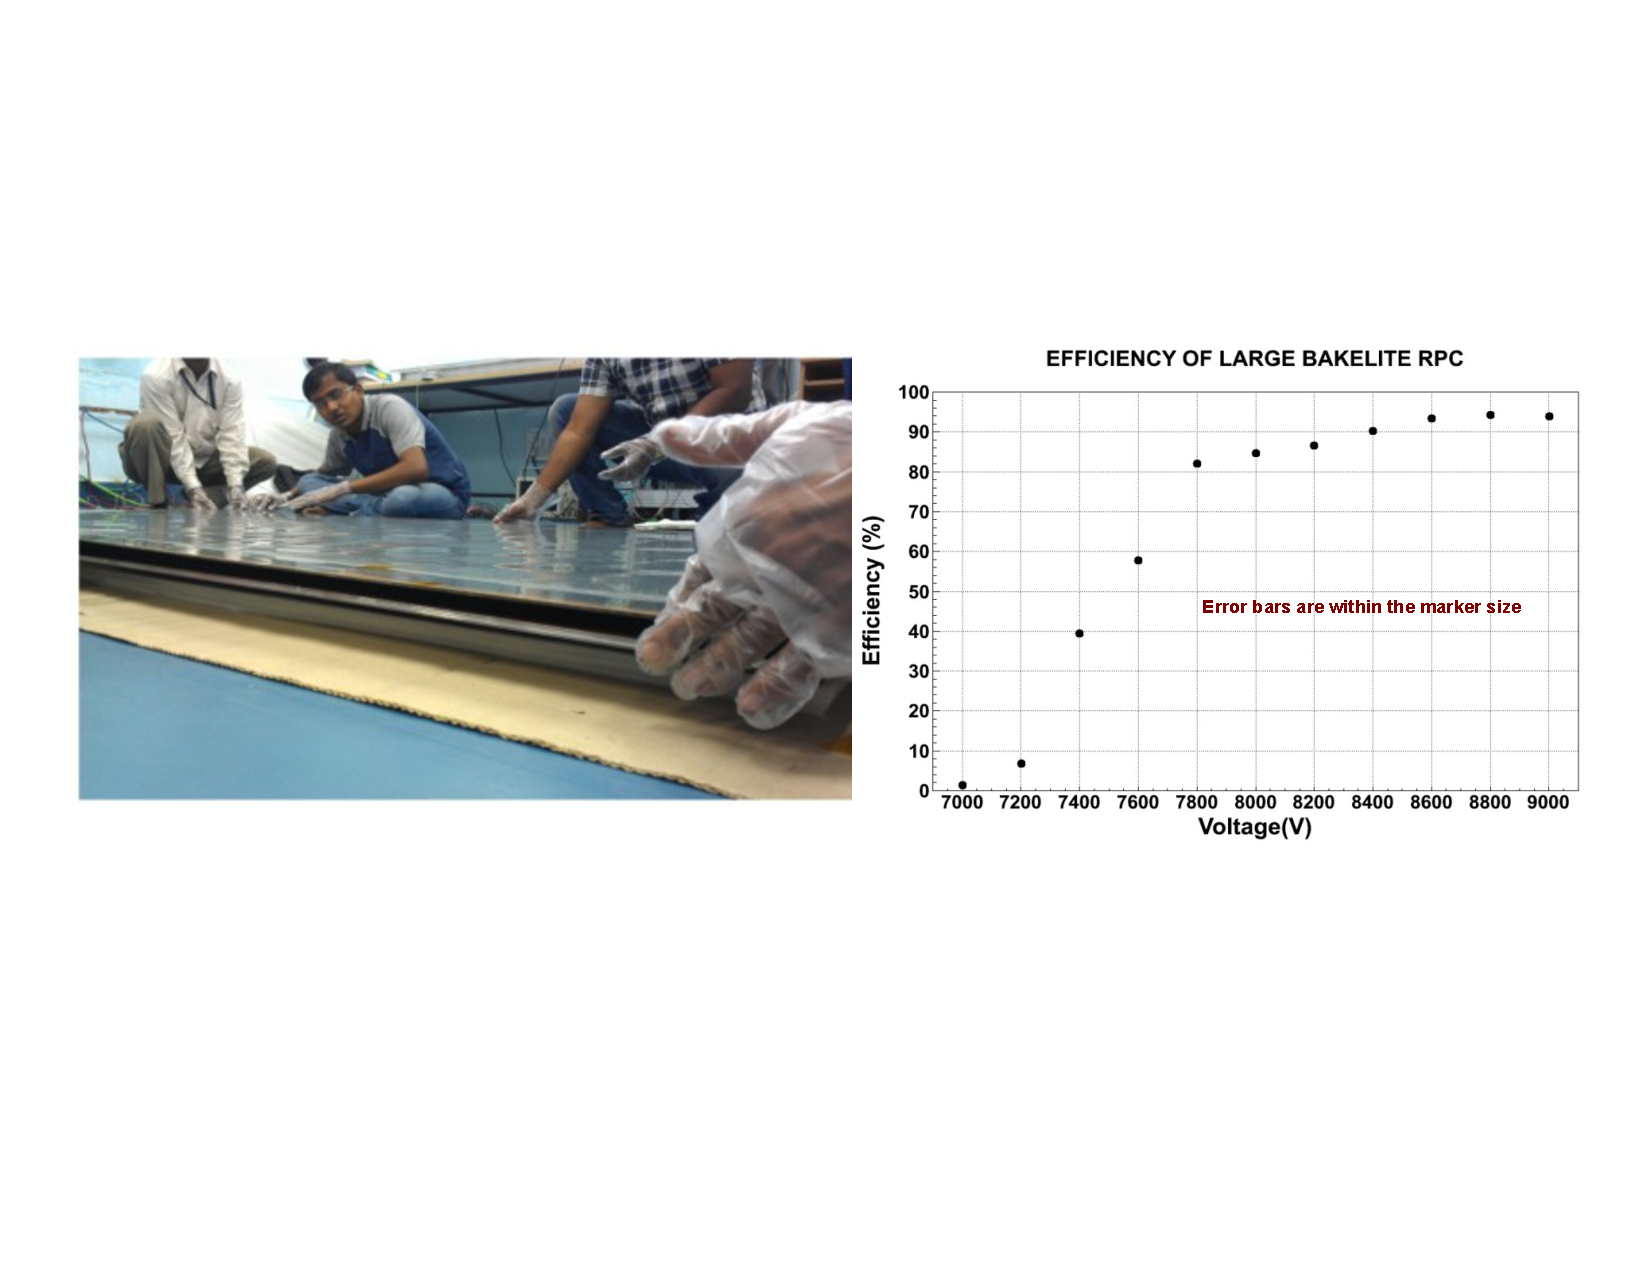
\includegraphics[width=\textwidth]{RPC_Prototype} % [width=5in,angle=90] <-- was too small
\end{cdrfigure}

The nominal dimensions of all RPC modules will be 1~m $\times$ 2~m with
active areas of 96~cm $\times$ 196~cm. Each
module has 256 X strips
at 7.65-mm pitch and 128 Y strips at 7.5-mm pitch. The modules
will be grouped into trays, each containing six modules, and the trays will
be sufficiently wide to allow overlapping modules. 
The downstream MuID will contain five steel planes of 
overall dimensions
6 $\times$ 6 $\times$ 0.2~m$^3$ (283.5~t)
and five RPC planes, while the upstream MuID will contain three steel
planes (170.1~t) of dimensions 6 $\times$ 6 $\times$ 0.2~m$^3$ and three RPC planes. The barrel MuID will contain
24 planes (three layers $\times$ eight sides) of RPCs. The RPCs will have a total thickness 
of 15~mm and a gap width of 2~mm. One possible gas mixture could be %composed, for example,
of Ar (75\%), tetraflouroethane (20\%), isobutane (4\%),
and sulphurhexaflouride (1\%). 
Figure~\ref{fig:FGT_RPC} shows a schematic drawing of an RPC module. 



%%%%%%%%%%%%%%%%%e
\subsection{Instrumentation}
\label{cdrsec:detectors-nd-ref-fgt-instrum}

The instrumentation includes both fast readout electronics for the subdetectors
and the slow control ($\mathcal{O}$ seconds) of the subdetectors, involving monitoring the humidity, 
temperature, gas pressure, etc.
There is considerable synergy in the information gathered in the STT, ECAL and MuID. 
Both the STT and ECAL are required to measure the total charge and the time associated with a 
given hit. The MuID RPCs are required to provide the position and time associated with 
a traversing track. Similarly, the slow control of the subdetectors
share many features.

The electronics for the three subsystems, STT, MuID, and ECAL, are all ``fast'' systems, 
i.e., all of the signals are in the few-to-10 nanosecond range. 
The requirements for each system are very similar: a fast output and both an ADC  
and a TDC on each channel.  Additionally, for the STT straw tubes it 
is desirable to wave-form digitize the analog signal in order to enhance the ability to separate 
the ionization signal from the transition radiation signal. 
The total channel count in FGT is 433,152 channels, as shown in Table~\ref{tab:elect_ch}.  

\begin{cdrtable}[Number of electronics channels for each of the
three detector systems]{ll}{elect_ch}{The number of electronics channels for each of the
three detector systems}
Detector&\# of Channels\\ \toprowrule
STT & 215,040 \\  \colhline
ECAL & 52,224 \\  \colhline
MuID & 165,888 \\
\end{cdrtable}

Recently, an interesting new ASIC development for an upgrade to the ATLAS muon system at the LHC
has come out of BNL), the VMM2 chip. %\fixme{add G. DeGeronimo at BNL ref} 
 It handles 64 channels and produces both fast ADC and TDC outputs.
It has been fabricated and tested and should be ready by 2017, long before it will be needed for DUNE.

To maintain a low level of 
humidity and to maintain a desired temperature, both STT and ECAL subdetectors
will have dry nitrogen circulating within their outer layers.  Magnet coils are cooled by water, 
while the magnet yokes are instrumented with RPCs that must remain dry. Continuous control of 
humidity in all these detectors is needed.
Temperature must also be continuously monitored in all of the subdetectors
in order for the electronics to not overheat. 
To ensure that the magnet does not overheat, the water flow (pressure gradient) will be continuously monitored.  
Also, all power sources instrumenting the FGT and its readout need to be monitored for 
appropriate voltage and current.

Gas leaks need to be monitored in the STT and MuID.
The STT will employ Xe gas, which helps with the measurement of transition radiation.
Xe gas is expensive and, hence, will be recirculated; leak-monitoring is particularly important here.   
The requirement on leaks is less 
stringent for the RPCs, which have less expensive gas.

The water flow (pressure gradient) will be continuously monitored in order to ensure 
that the magnet does not overheat. 

